\documentclass{llncs}

\usepackage[italian]{babel}
\usepackage[utf8]{inputenc}
% \usepackage{hyperref}
\usepackage{graphicx}

\usepackage[T1]{fontenc}
\usepackage{subcaption}
\captionsetup{compatibility=false}
%\usepackage{float}
\usepackage{amssymb}
\author{Giuseppe De Palma}

\title{Progetto Elaborazione Linguaggio Naturale: Tecniche di Clustering}
\institute{Alma Mater Studiorum - Università di Bologna \\
	\email{giuseppe.depalma@studio.unibo.it}\\
	\email{Matricola: 854846}
}
\newcommand{\acapo}{\vspace{0.5\baselineskip}\\}

\begin{document}
    \maketitle
		   
	\section{Introduzione}
	Il \textit{clustering} (o analisi dei gruppi) è una forma di \textit{machine learning} non supervisionato che permette di raggruppare in \textit{cluster} elementi non annotati
	dati in input. Un cluster è una collezione di oggetti ``simili'' tra loro che sono ``dissimili'' rispetto agli oggetti degli altri cluster. Questo tipo di machine learning è
	ottimo per partizionare un insieme di dati in diverse ``categorie'', quindi poter eseguire diverse analisi ed ottenere nuove informazioni.
	Applicazioni tipiche in cui il clustering viene molto usato è il riconoscimento di email di spam (le email a scopi pubblicitari o di frode), oppure per l'aggregazione di notizie (Google News ne è un esempio).
	\acapo
	Il clustering trova possibili applicazioni anche nel campo dell'elaborazione del linguaggio naturale. Oltre alle nuove possibili analisi
	sui corpora ed al fornire una visualizzazione grafica delle parole raggrupate, un interessante utilizzo è quello della \textbf{generalizzazione} delle parole.
	\acapo 
	Possiamo considerare i vari cluster delle classi di equivalenza. Per questo motivo, se avessimo un dataset su cui comporre i cluster fatto di frasi e parole, allora si potrebbe assumere che una
	qualche parola che compare in una frase può essere sostituita con un'altra dello stesso cluster lasciando intatta la correttezza della frase. 
	Ad esempio, se avessimo nel nostro dataset ``per Lunedì'', ``per Martedì'', ``per Mercoledì'', ``per Sabato'', ``per Domenica'', senza avere ``per Giovedì'' e ``per Vernedì'', e avessimo un cluster in cui 
	i giorni della settimana sono raggruppati insieme, allora potremmo generalizzare l'utilizzo della preposizione ``per'' con Giovedì e Vernedì.
	\acapo
	Il clustering, quindi, può essere molto utile anche nell'elaborazione del linguaggio naturale. Nel progetto in studio vengono testate le capacità di alcune tecniche di clustering
	da cui si derivano dei risultati per mostrarne le differenze, i pregi e i difetti. I dati utilizzati negli esperimenti, comunque, non sono parti di testo, ma semplici dataset di vettori numerici 2D in modo tale da poter facilmente 
	visualizzare i grafici relativi ai cluster e determinare le caratteristiche di ogni tecnica.
	\subsection{Outline}
	Nella prossima sezione vengono discussi i diversi algoritmi di clustering in studio, dove per ognuno sono descritte le proprietà, gli utilizzi e la logica dietro il loro funzionamento.
	In seguito è presentata la sessione sperimentale dove alcuni test e considerazioni sono mostrati. Infine si conclude spiegando le differenze più marcate tra le tecniche.
	\section{Clustering}
	Ci sono numerosi algoritmi per effettuare clustering, ma essi sono classificabili in poche tipologie: il clustering partizione e il clustering gerarchico.
	Il clustering partizionale consiste nell'ottenere dei cluster, di solito in modo iterativo, ma spesso senza determinare una vera relazione tra gli elementi. Si inizia con un insieme di cluster iniziale ed iterativamente
	si riassegnano gli oggetti nei giusti cluster. Il clustering gerarchico, invece, forma un albero (la gerarchia) degli elementi dove un nodo rappresenta un sotto-cluster del nodo padre e le foglie sono i singoli
	oggetti.
	\acapo
	Un'altra importante distinzione tra gli algoritmi di clustering è il \textit{soft clustering} e \textit{hard clustering}. Nel primo caso, ogni oggetto può essere assegnato a più cluster secondo un qualche
	grado di appartenenza, mentre nel secondo caso ogni oggetto è assegnato ad un unico cluster. In questo progetto vedremo quattro diversi algoritmi, due della classe di clustering gerarchico, due del clustering partizionale.
	I primi tre eseguono hard clustering mentre l'ultimo (EM) soft clustering.
	\acapo
	Di seguito sono elencati i metodi implementati e testati:
	\begin{itemize}
		\item Clustering \textbf{gerarchico}
		\begin{enumerate}
			\item Aggregativo
			\item Divisivo
		\end{enumerate}

		\item Clustering \textbf{partizionale}
		\begin{enumerate}
			\item K-means
			\item EM
		\end{enumerate}
	\end{itemize}
	
	\subsection{Gerarchico}
	Andando più in dettaglio sulle diverse tecniche, abbiamo detto che la prima classe di clustering permette di creare degli alberi con i cluster e sotto-cluster. 
	Questo può essere ottenuto con un approcco \textit{bottom-up} che è il clustering \textbf{aggregativo},
	il quale inizia dai singoli oggetti e ne raggruppa i più simili, per poi raggruppare i gruppi più simili e così via, fino ad ottenere un unico gruppo
	che sarà la radice dell'albero. Un altro approccio è quello \textit{top-down}, il clustering \textbf{divisivo}, che in modo inverso dal precedente parte 
	dal gruppo comprendente tutti gli elementi e lo divide in sotto-gruppi in modo da massimizzare la similarità intrinseca dei gruppi, 
	fino ad arrivare ai singoli elementi.
	\begin{figure}[h]
		\centering
		\begin{subfigure}[b]{\textwidth}
		   	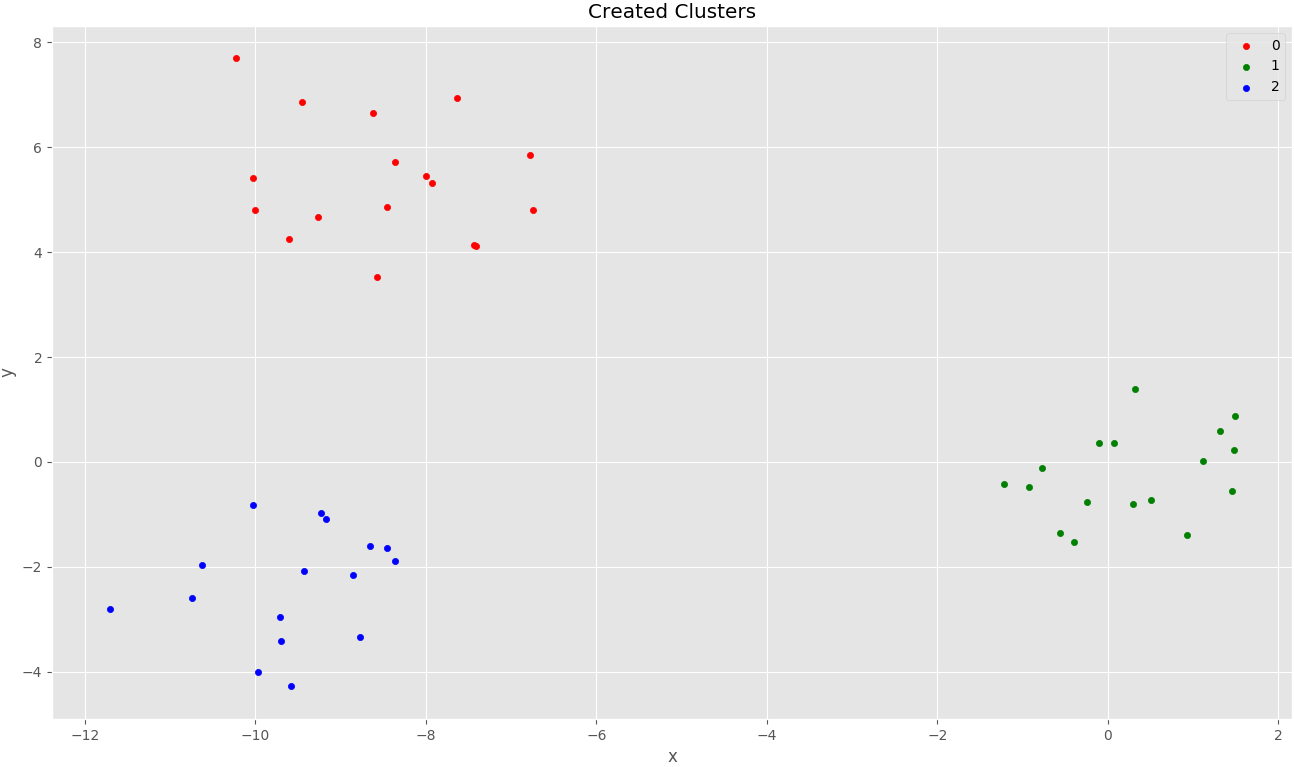
\includegraphics[width=\linewidth]{immagini/created_cluster_dend_ex.png}
		   	\label{fig:1} 
		\end{subfigure}
		
		\begin{subfigure}[b]{\textwidth}
			\centering
		   	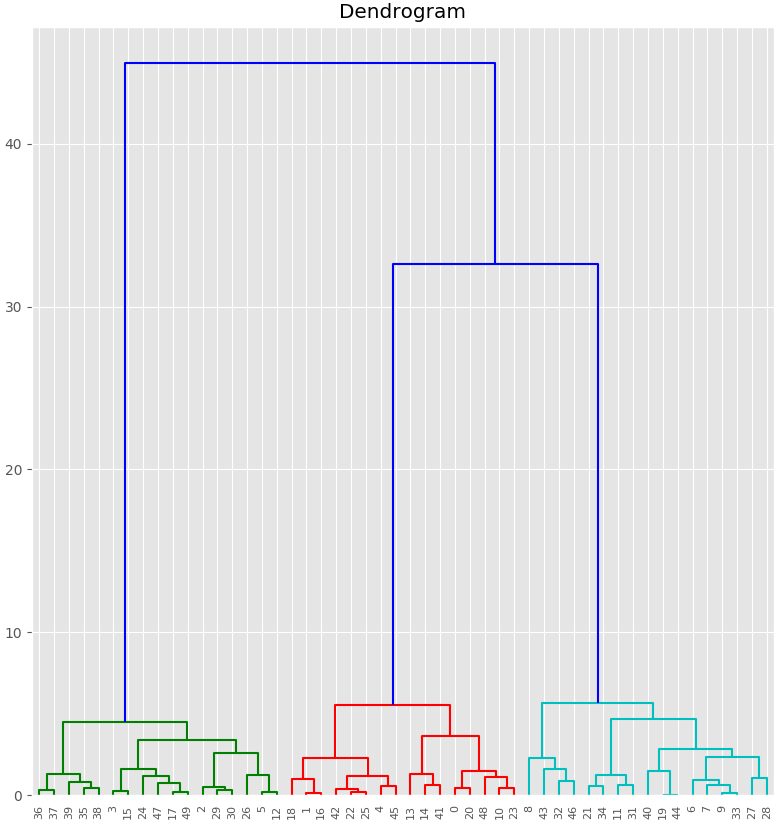
\includegraphics[scale=0.5]{immagini/dendrogam_example.png}
		   	\label{fig:2}
		\end{subfigure}
		\caption{(a) insieme di 50 punti pre-divisi in 3 gruppi distinti, su cui si applica il clustering aggregativo con la funzione di 
		similarità ward. Se ne ricava un dendogramma, in (b), che mostra le relazioni dei dati. Si noti come tagliando orizzontalmente il cluster per le linee verticali più alte dove non appaiono linee orizzontali, rimangono proprio 3 sotto-cluster.}
		\label{ex:dendrogram}
	\end{figure}
	\clearpage
	L'albero che si ottiene può essere visualizzato tramite un dendrogramma, come nella figura \ref{ex:dendrogram}.
	Questo diagramma ci mostra le relazioni gerarchiche tra gli oggetti, infatti il suo principale utilizzo è quello di 
	mostrare il modo migliore di organizzare i cluster. 
	\acapo
	Concentrandosi sulle linee verticali possiamo capire il numero ottimale di cluster
	da prefissare, siccome l'asse $y$ misura la somiglianza dei cluster, mentre l'asse $x$ rappresenta gli oggetti e i cluster.
	Disegnando una linea orizzontale che ``taglia'' il dendrogramma, si afferma che i sotto-cluster al di sotto di questa linea saranno i raggruppamenti finali.
	Poichè linee verticali corte rappresentano gradi di similarità più alti tra gruppi, tagliando il dendrogramma per le linee verticali più alte che sono libere da 
	linee orizzontali (quando c'è una unione di cluster), si ha il numero di cluster ottimale a cui assegnare gli elementi,

	\subsubsection{Aggregativo}
	Questo tipo di clustering è realizzato tramite un algoritmo \textit{greedy} che prende in input un insieme di dati $S$, da cui ogni oggetto è considerato essere un piccolo cluster da un solo elemento.
	Ad ogni passo l'algoritmo determina i due cluster più simili e li unisce in un nuovo cluster. L'algoritmo termina
	quando il cluster contenente tutti gli elementi di $S$ viene formato, il quale sarà l'unico cluster rimanente.
	I modi in cui si possono determinare la similarità dei cluster sono molteplici. L'algoritmo fa uso di una funzione di similarità per calcolare quanto due cluster sono simili tra di loro.
	Ne esistono diverse, ad esempio alcune molto utilizzate sono:
	\begin{itemize}
		\item \textit{single link}: ottiene la similarità di due membri \textbf{più} simili da due cluster diversi, rispettivamente;
		\item \textit{complete link}: ottiene la similarità dei due membri \textbf{meno} simili da due cluster diversi, rispettivamente;
		\item \textit{group-average}: ottiene la similarità media tra i membri di due cluster.
		\item \textit{ward}: ottiene la similarità in base al costo di unione di due cluster. Questo costo è ottenuto calcolando la somma dei prodotti tra gli elementi di due cluster e i loro centroidi. 
	\end{itemize}
	Nonostante le funzioni di similarità possano differire anche ampiamente, una proprietà che tutte devono avere è la monotonia. Per un insieme di dati $S$ e una funzione di similarità $sim$:
	\begin{center}
		$\forall c, c', \hat{c} \subseteq S$. $min(sim(c, c’), sim(c, \hat{c})) \ge sim(c, c’ \cup \hat{c})$
	\end{center}
	Questo perché l'operazione di unione garantisce	di non aumentare la similarità, quindi una funzione che non obbedisce a questa condizione
	rovinerebbe la gerarchia in quanto cluster non simili, piazzati in parti lontane nell'albero, potrebbero
	ritrovarsi ad essere simili in unioni successive e perciò l'essere vicini nell'albero non corrisponderebbe più al concetto di similarità.

	\subsubsection{Divisivo}
	Come per la controparte aggregativa, dietro il clustering divisivo c'è un algoritmo greedy. Invece di iniziare dai singoli elementi, si inizia dal cluster contenente tutti gli oggetti. Ad ogni iterazione
	si determina quale cluster è quello \textbf{meno} coerente e lo si divide in due. Come prima si utilizzano funzioni di similarità, poichè due cluster con oggetti simili sono più coerenti
	di cluster con oggetti non simili. L'operazione di divisione di un cluster è anch'essa una operazione di clustering, poichè bisogna trovare
	due sotto-cluster. Qualsiasi tecnica di clustering può essere usata per la divisione, anche il clustering aggregativo, ma spesso si utilizza K-means (come in questo progetto).
	Per queste ragioni il clustering divisivo è solitamente meno usato.
	
	\subsection{Partizionale}
	Diversamente dal clustering appena discusso, gli algoritmi per quello partizionale spesso
	iniziano con una divisione casuale del dataset in vari cluster, per poi raffinarli passo dopo passo attraverso 
	la ricollocazione degli oggetti. Da questo procedimento sorgono varie domande: 
	\begin{enumerate}
		\item Quando fermarsi con la ricollocazione?
		\item In quanti cluster dividere il dataset?
		\item In che modo si seleziona il miglior cluster in cui ricollocare un elemento?
	\end{enumerate} 
	Quando fermarsi può essere determinato tramite una metrica sulla qualità dei cluster. Questa può essere una funzione 
	di similarità come la group-average (che va a toccare tutti i cluster) e finchè il risultato incrementa di molto, si continua la procedura.
	\acapo
	La stessa metrica può essere utilizzata per rispondere alla seconda domanda. In alcuni casi possiamo già avere
	delle informazioni sul corretto numero di cluster da creare, oppure decidiamo arbitrariamente in quanti cluster dividere il dataset.
	In altri casi invece, possiamo dividere i dati in $k$ cluster osservando l'andamento della metrica.
	Per capire un buon numero di cluster da avere, bisogna vedere in quale transizione c'è un 
	incremento sostanziale da $k-1$ a $k$ cluster e un piccolo incremento da $k$ a $k+1$ cluster.
	Trovando un numero $k$ di cluster che abbia questa proprietà, possiamo avere in modo automatico una buona partizione del dataset.
	\acapo
	Per l'ultima questione, sono gli algoritmi per il clustering partizionale che si occupano di come ricollocare gli oggetti, che ora verranno 
	presentati.
	\subsubsection{K-means}
	K-means è un algoritmo di hard clustering che definisce i cluster attraverso i loro punti centrali.
	Partendo da dei centroidi iniziali, iterativamente si assegna ogni oggetto al cluster il cui centroide è
	il più vicino, calcolato tramite la distanza euclidea. Una volta che tutti gli elementi sono stati assegnati, si ricalcolano i punti centrali di tutti
	i cluster e si ripete il procedimento di assegnazione così da raffinare il clustering.

	\subsubsection{EM}
	L'algoritmo EM (Expectation-Maximization) è definibile come la versione di K-means per il soft clustering.
	In quest'algoritmo possiamo vedere ogni cluster come una distribuzione di probabilità (in questo progetto vedremo l'algoritmo EM con \textit{Gaussian mixture model}).
	L'idea è quindi di alternare due step: l'Expectation step dove accade il calcolo delle probabilità per ogni oggetto di essere stato generato da ognuna delle distribuzioni 
	(in K-means questo è analogo ad assegnare ogni punto ad un cluster). 
	Successivamente c'è il Maximization step, in cui si massimizzano i parametri delle distribuzioni e degli oggetti (pesi, covarianza, medie) così da poter ripetere il primo step
	per raffinare le probabilità. 
	L'equivalente in K-means è muovere i punti centrali dei cluster per poi procedere con un'altra riallocazione.

	\section{Sessione Sperimentale}
	In questa sezione verranno mostrati vari esperimenti per sottolineare le differenze tra i quattro metodi presentati. Sono stati effettuati diversi test usando diversi dataset di vettori 2D, 
	così da facilmente visualizzare i risultati con grafici. Per l'algoritmo di clustering aggregativo è stato scelto di usare la funzione di similarità ward. 
	Per il clustering	divisivo viene usato K-means per creare 2 cluster a partire da un cluster più grande, che è lo step di divisione. Per scegliere quale cluster dividere, 
	sono state vagliate diverse possibilità:
	
	\begin{itemize}
		\item Un approccio comune è quello di selezionare il cluster con la massima cardinalità. Questo dà priorità alla produzione di cluster bilanciati rispetto alle dimensioni;
	
		\item Un altro modo è calcolare il raggio di ogni cluster, il quale è la massima distanza tra i punti e il centroide. Quindi si seleziona il cluster con il raggio maggiore;
			
		\item Un altro approccio è calcolare il diametro di ogni cluster, il quale è la massima distanza tra ogni coppia di punti di un cluster.
			Come prima, si va a scegliere il cluster che ha il diametro maggiore.
	\end{itemize}
	Data la sua immediatezza, si è scelto di utilizzare il primo approccio.
	\acapo
	Vengono ora mostrati dei test che rappresentano i diversi esperimenti eseguiti. Prima viene mostrato un dataset e dei testi dove il clustering 
	aggregativo e divisivo sono stati adoperati. In seguito i due metodi sono presentati i risultati dei due metodi di clustering partizionale. Infine sarà dato un quadro
	generale delle differenze riscontrate.
	
	\clearpage
	\subsection{Aggregativo e Divisivo}
	Il primo dataset, mostrato in figura \ref{c:5_c}, contiene 1000 elementi distintamente raggruppati con colori diversi in 5 diverse zone, così che sarà ovvio quali cluster dovrebbero essere formati.
	\begin{figure}[h]
		\centering
		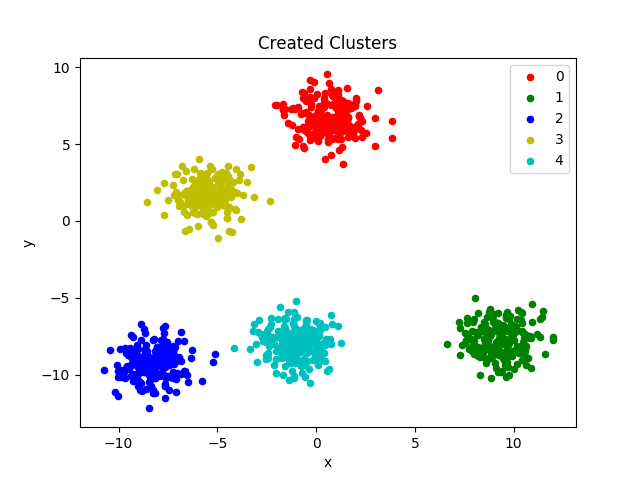
\includegraphics[scale=.35]{immagini/5_clusters.png}
		\caption{Dataset di 1000 elementi raggruppati in 5 diverse zone, etichettati con colori diversi. Questi saranno i cluster che le varie tecniche formeranno.}
		\label{c:5_c}
	\end{figure}\\
	Una prima applicazione delle due tecniche è stata quella di lanciare le procedure prefissando il numero di cluster da ottenere. 
	In figura \ref{hier_normal:test} e \ref{hier:test} sono mostrati alcuni risultati.
	Per entrambe le tecniche, se richiesto di trovare esattamente il numero di cluster che il dataset prevede (in questo caso 5),
	allora vengono identificati in modo molto simile i vari gruppi. La tecnica aggregativa è magari poco più precisa per quegli elementi ai confini tra due diversi cluster. 
	\begin{figure}[h]
		\centering
		\begin{subfigure}{.45\textwidth}
		  \centering
		  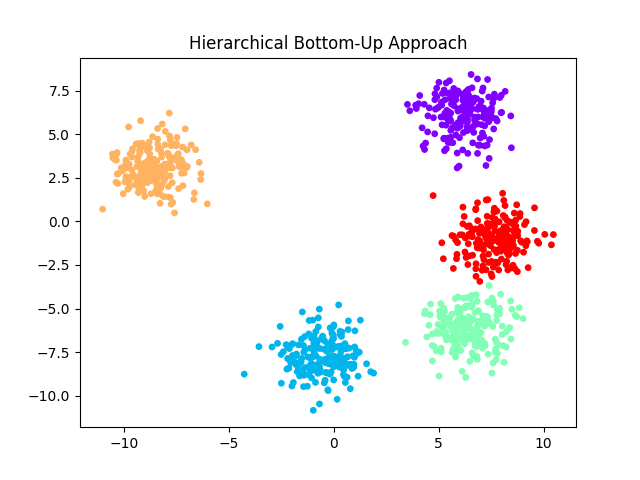
\includegraphics[width=\linewidth]{immagini/5_clusters_agg.png}
		  \caption{Aggregativo per i 5 cluster.}
		  \label{hier_normal:a}
		\end{subfigure}%
		\begin{subfigure}{.45\textwidth}
		  \centering
		  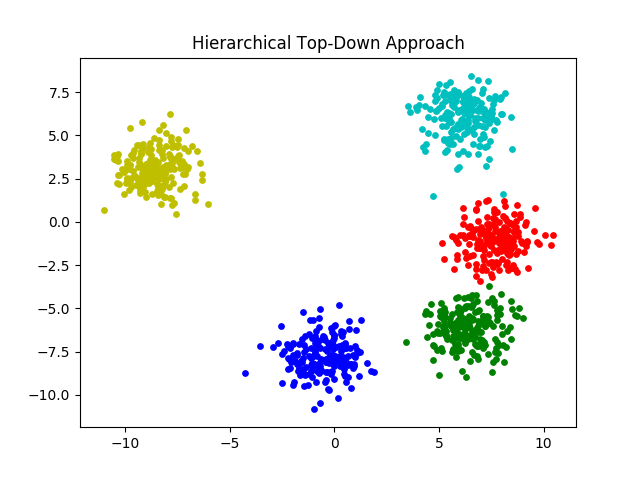
\includegraphics[width=\linewidth]{immagini/5_clusters_div.png}
		  \caption{Divisivo per i 5 cluster.}
		  \label{hier_normal:b}
		\end{subfigure}
		\caption{I risultati delle due tecniche per il clustering gerarchico sul dataset mostrato in figura \ref{c:5_c}.
		La formazione dei cluster è molto simile per entrambi gli algoritmi, i gruppi principali identificati sono gli stessi.
		Piccole differenze per gli elementi molto vicini a 2 o più cluster.}
		\label{hier_normal:test}
	\end{figure}
	\\
	Invece iniziano ad esserci delle differenze anche sostanziali quando si vuole avere un numero minore o maggiore di cluster.
	Le figure \ref{hier:a} e \ref{hier:b} mostrano due istanze in cui si vogliono 3 cluster. In questo caso i cluster trovati sono tutti e 3 diversi per i due algoritmi.
	Spesso pochi, separati cluster possono risultare diversi, ma a seconda dell'approccio utilizzato per la scelta del cluster da dividere,
	i risultati possono differire molto da ciò che si ottiene con la tecnica aggregativa.
	\acapo
	Si è poi raddoppiato il numero di cluster voluto, da 5 a 10, i cui risultati sono mostrati in \ref{hier:c} e \ref{hier:d}.
	Entrambe le tecniche hanno seguito la strada di dividere in due ciascuna delle 5 zone dove sono raggruppati gli elementi, ottenendo 10 cluster.
	Qui si riesce a notare bene come il clustering divisivo faccia dei tagli decisamente più netti per dividere i gruppi.
	\begin{figure}[h]
		\begin{subfigure}{.5\textwidth}
		  \centering
		  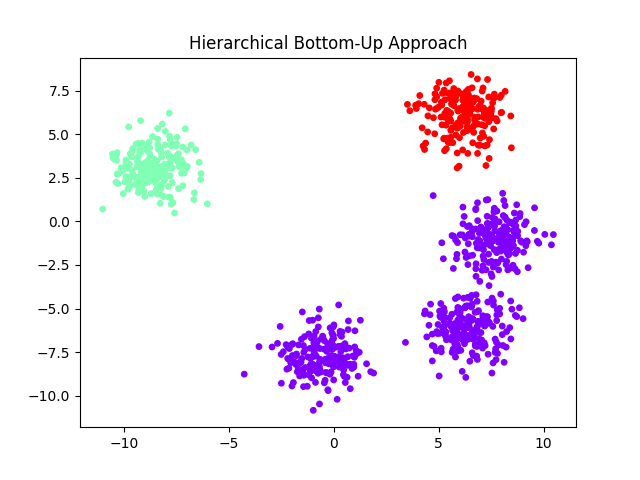
\includegraphics[width=\linewidth]{immagini/5_clusters_agg_3.png}
		  \caption{Aggregativo per 3 cluster.}
		  \label{hier:a}
		\end{subfigure}%
		\begin{subfigure}{.5\textwidth}
		  \centering
		  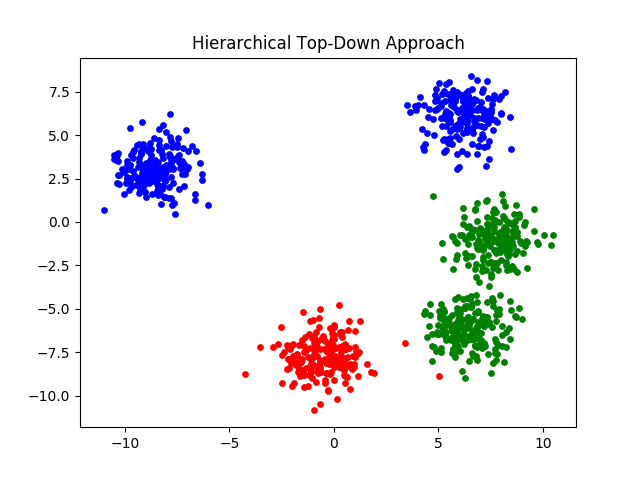
\includegraphics[width=\linewidth]{immagini/5_clusters_div_3.png}
		  \caption{Divisivo per 3 cluster.}
		  \label{hier:b}
		\end{subfigure}
		\begin{subfigure}{.5\textwidth}
			\centering
			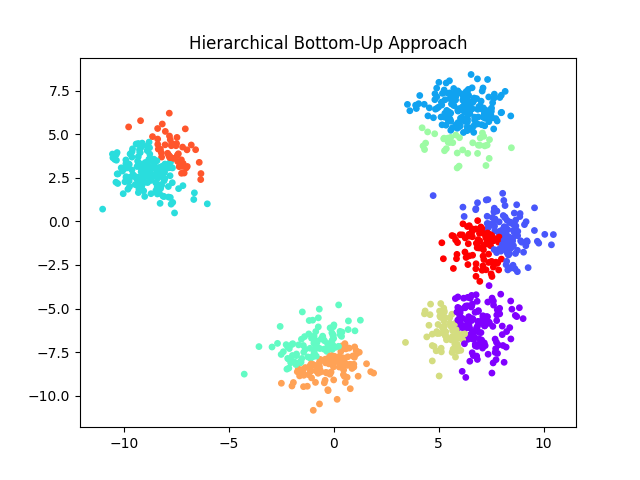
\includegraphics[width=\linewidth]{immagini/5_clusters_agg_10.png}
			\caption{Aggregativo per 10 cluster.}
			\label{hier:c}			
		  \end{subfigure}
		  \begin{subfigure}{.5\textwidth}
			\centering
			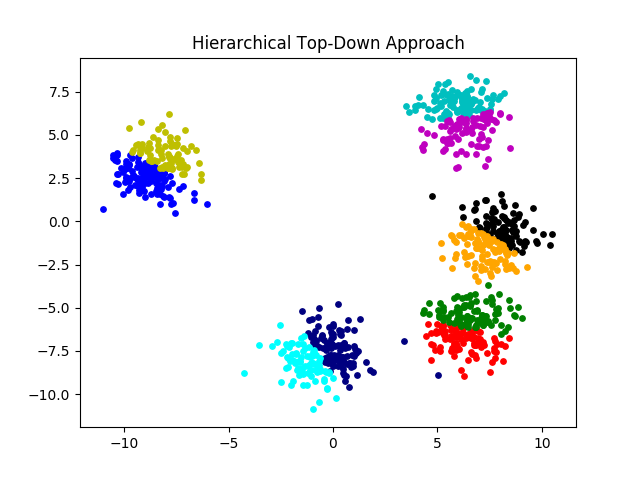
\includegraphics[width=\linewidth]{immagini/5_clusters_div_10.png}
			\caption{Divisivo per 10 cluster.}
			\label{hier:d}			
		  \end{subfigure}
		\caption{Sempre con lo stesso dataset (dalla figura \ref{c:5_c}), sono qui mostrati i risultati del clustering gerarchico prefissando
		l'identificazione di 3 cluster, (a) e (b), e 10 cluster, (c) e (d), invece di 5.}
		\label{hier:test}
	\end{figure}
	\clearpage
	Oltre queste differenze, anche il tempo richiesto di esecuzione è stato abbastanza diverso tra le due tecniche. Il clustering aggregativo è stato
	decisamente più veloce nel completare i calcoli. Questo è chiaramente dovuto al non utilizzare una seconda tecnica di clustering per formare nuovi cluster, 
	cosa che invece il clustering divisivo fa per dividere gli elementi.

	\subsection{K-means ed EM}
	Una prima differenza sostanziale di K-means, anche con le tecniche precedenti, è la velocità di esecuzione. In tutti i test il calcolo dei cluster è stato immediato.
	Decisamente un vantaggio non da poco. 
	\acapo
	In figura \ref{part_norm:test} vengono mostrati i due algoritmi applicato al dataset precedente. K-means non solo è stato piuttosto veloce, ma ha formato gli stessi 5 cluster descritti dal dataset.
	EM invece, essendo un algoritmo di soft clustering, mostra come gli elementi rientrino in più di un cluster. Gli elementi in giallo appartengono ad un unico cluster, essendo essi ben separati dagli altri. 
	Per il resto invece, essendo tra loro più vicini, non c'è una divisione ovvia. Anzi, molti elementi fanno parte di due o più cluster con probabilità molto simili. 
	Ad esempio, i punti rossi che sono molto vicini ai punti blu hanno una probabilità molto alta sia per il cluster blu che per il rosso, ma di poco sono stati classificati come rossi.
	\begin{figure}[h]
		\centering
		\begin{subfigure}{.45\textwidth}
		  \centering
		  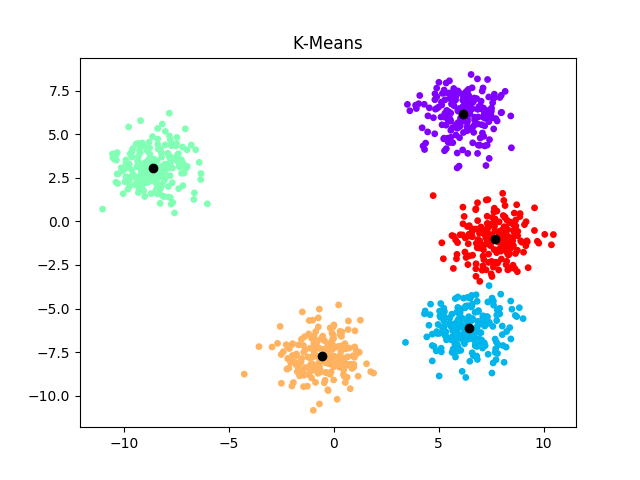
\includegraphics[width=\linewidth]{immagini/5_clusters_kmeans.png}
		  \caption{K-means per i 5 cluster.}
		  \label{part_norm:a}
		\end{subfigure}%
		\begin{subfigure}{.45\textwidth}
		  \centering
		  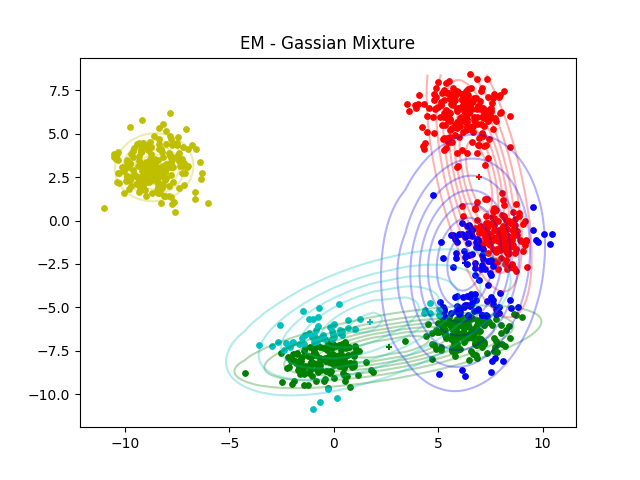
\includegraphics[width=\linewidth]{immagini/5_clusters_gmm.png}
		  \caption{EM per i 5 cluster.}
		  \label{part_norm:b}
		\end{subfigure}
		\caption{I risultati delle due tecniche per il clustering partizionale sul dataset mostrato in figura \ref{c:5_c}.
		In (a) K-means riesce a partizionare gli elementi esattamente come nel dataset originale, i punti neri sono i centroidi. In (b) EM invece forma 1 cluster ben definito (colore giallo), mentre con gli altri 4 c'è un
		netto soft clustering, dove alcuni elementi fanno parte perfino di 3 cluster diversi.}
		\label{part_norm:test}
	\end{figure}\\
	Anche per queste due tecniche si è voluto testare l'identificazione prima di 3 cluster, poi di 10. In \ref{part:a} K-means trova 3 ottimi cluster, di nuovo diversi da quelli trovati dalle tecniche gerarchiche.
	Uno è chiaramente ben separato dagli altri, mentre gli altri due sono ognuno due gruppi vicini tra di loro. Questo è probabilmente il miglior modo per suddividere quel dataset in 3 cluster. 
	Invece in \ref{part:b} EM suddivide il dataset in modo ulteriormente diverso, però i 4 gruppi a destra in realtà condividono l'appartenenza in 2 cluster.
	\\
	\begin{figure}[h]
		\begin{subfigure}{.5\textwidth}
		  \centering
		  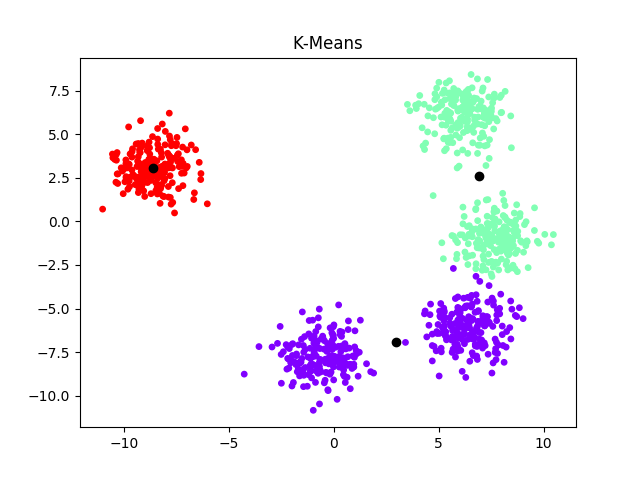
\includegraphics[width=\linewidth]{immagini/5_clusters_kmeans_3.png}
		  \caption{K-means per 3 cluster.}
		  \label{part:a}
		\end{subfigure}%
		\begin{subfigure}{.5\textwidth}
		  \centering
		  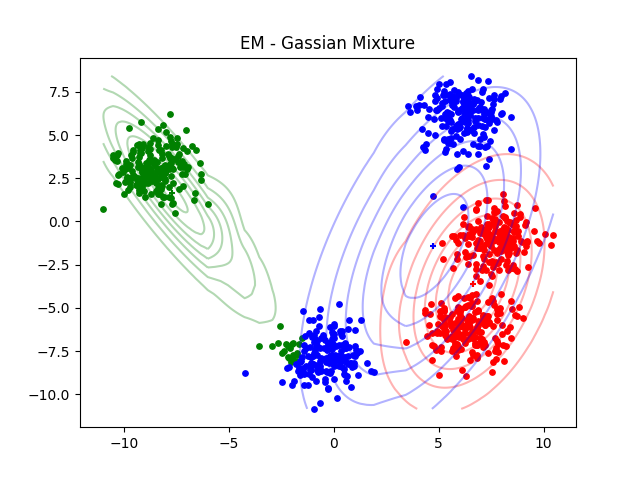
\includegraphics[width=\linewidth]{immagini/5_clusters_gmm_3.png}
		  \caption{EM per 3 cluster.}
		  \label{part:b}
		\end{subfigure}
		\begin{subfigure}{.5\textwidth}
			\centering
			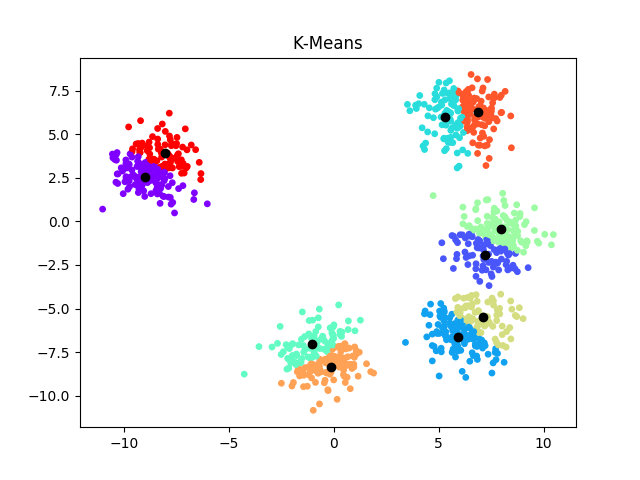
\includegraphics[width=\linewidth]{immagini/5_clusters_kmeans_10.png}
			\caption{K-means per 10 cluster.}
			\label{part:c}			
		  \end{subfigure}
		  \begin{subfigure}{.5\textwidth}
			\centering
			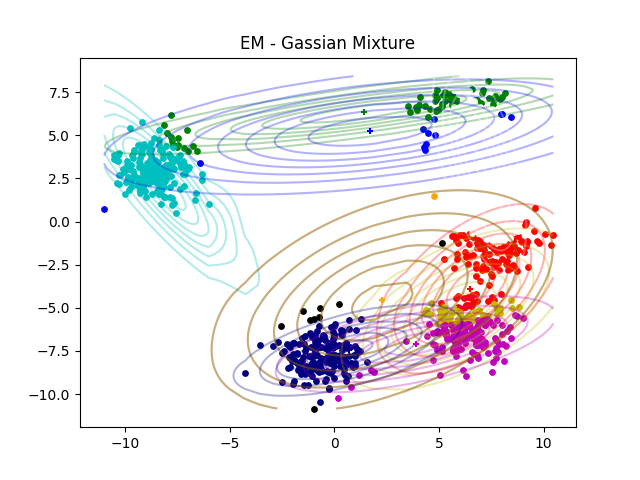
\includegraphics[width=\linewidth]{immagini/5_clusters_gmm_10.png}
			\caption{EM per 10 cluster.}
			\label{part:d}			
		  \end{subfigure}
		\caption{I Risultati del clustering partizionale prefissando
		l'identificazione di 3 cluster, (a) e (b), e 10 cluster, (c) e (d).}
		\label{part:test}
	\end{figure}\\
	Per il caso dei 10 cluster da creare, si nota come in \ref{part:c} c'è una divisione abbastanza netta come nel caso del clustering divisivo, il che è prevedibile in quando la tecnica divisiva 
	implementata utilizza K-means. Da EM, invece, non traspare una chiara struttura dei cluster quando se ne richiede un alto numero, sopratutto se gli elementi sono ben distinti in un numero inferiore di gruppi.
	Questo ci dice che, ignorando per il momento i tempi di esecuzione più lunghi, in una applicazione concreta questa tecnica va usata più che altro quando c'è un reale bisogno di fare soft clustering
	con un numero appropriato di cluster da identificare.  
	\clearpage
	\section{Conclusioni}
	Tenendo conto sia del funzionamento degli algoritmi sia di questi ed altri test, si è notato che il clustering gerarchico può essere più adatto per analisi più dettagliate, come quando c'è un
	bisogno di informazioni maggiori sulle relazioni tra gli elementi. L'approccio aggregativo è più facile da implementare di quello divisivo, ma entrambi hanno i propri casi d'uso. Sono però meno
	efficienti del clustering partizionale, dove K-means è il migliore. Per questo motivo quando c'è un reale bisogno di efficienza, senza dubbio il clustering partizionale è da scegliere. Inoltre,
	K-means è anche l'algoritmo concettualmente più semplice. Se i suoi risultati sono già sufficienti allora è un'ottima scelta. Infine EM ha i suoi casi d'uso, ad esempio quando è utile
	fare soft clustering oppure bisogna usare modelli probabilistici anche complessi, anche con dataset sofisticati e non necessariamente rappresentati in spazi euclidei 
	(cosa richiesta da K-means).



\begin{thebibliography}{9}
	\bibitem{manning} 
	Christopher D. Manning, Hinrich Scht{\"u}ze

	\textit{Foundations of Statistical Natural Language Processing}. 
	The MIT Press Cambridge, Massachusetts 1999.
	
	\bibitem{clmerg} 
	Chris Ding, Xiaofeng He
	\textit{Cluster merging and splitting in hierarchical clustering algorithms}.
	University of California, Berkeley,
\end{thebibliography}
	
	
\end{document}
